\documentclass[conference]{IEEEtran}
\IEEEoverridecommandlockouts
% The preceding line is only needed to identify funding in the first footnote. If that is unneeded, please comment it out.
\usepackage{cite}
\usepackage{amsmath,amssymb,amsfonts}
\usepackage{algorithmic}
\usepackage{graphicx}
\usepackage{textcomp}
\usepackage{xcolor}
\usepackage{tikz}
\usepackage{multirow}
\usepackage[hidelinks]{hyperref}
\usepackage{multirow}
\usepackage[normalem]{ulem}
\usepackage{makecell}
\useunder{\uline}{\ul}{}
\usetikzlibrary{positioning}

\usepackage[acronym,toc]{glossaries}

\makeglossaries

\def\BibTeX{{\rm B\kern-.05em{\sc i\kern-.025em b}\kern-.08em
    T\kern-.1667em\lower.7ex\hbox{E}\kern-.125emX}}
\begin{document}

\title{Video Super-Resolution using GANs\\
\thanks{978-1-6654-5992-1/22/31.00 ©2023 IEEE}
}

\author{\IEEEauthorblockN{1\textsuperscript{st} Oleh Pomazan}
\IEEEauthorblockA{\textit{Department of Software Engineering} \\
\textit{University of Europe for Applied Sciences}\\
oleh.pomazan@ue-germany.de}
% \and
% \IEEEauthorblockN{2\textsuperscript{nd} Given Name Surname}
% \IEEEauthorblockA{\textit{dept. name of organization (of Aff.)} \\
% \textit{name of organization (of Aff.)}\\
% City, Country \\
% email address or ORCID}
% \and
% \IEEEauthorblockN{3\textsuperscript{rd} Given Name Surname}
% \IEEEauthorblockA{\textit{dept. name of organization (of Aff.)} \\
% \textit{name of organization (of Aff.)}\\
% City, Country \\
% email address or ORCID}
}

% set path where images are stored
\graphicspath{{./img/}}

\maketitle


\begin{abstract}
    Video super-resolution is used to produce high-resolution video frames from the given low-resolution video frames, which can be used in a variety of vision tasks, including video restoration and enhancement, within the entertainment industry and streaming services. \acrfullpl{gan} are widely used for the super-resolution problems and SRGAN \cite{srgan_2016} is the most popular GAN model for \acrfull{sisr}. The SRGAN model uses a complex loss function consisting of pixel-wise \acrfull{mse}, perception, adversarial and total-variation parts. The effects of different components of the loss function on the SRGAN performance were studied by many authors \cite{esrgan_2018,srgan_2016,weighted_srgan_2021} but the role of total-variation loss is not well studied in the context of \acrshort{sisr}.

    In this thesis we study the effect of \acrfull{tv} loss on the performance of SRGAN model in the context of applying \acrlong{sisr} for video frames. The optimal range of the \acrshort{tv} loss weights was found to be between $10^{-8}$ and $10^{-6}$. Larger values of the \acrshort{tv} loss weight causes significant degradation of performance metrics and visible smoothing of the super-resolved frames.
    
    While the SRGAN model produces high-quality super-resolved images using a single low-resolution frame, it does not utilize additional information from the previous and next frames of the video. Therefore, we investigate the SRGAN model in terms of temporal consistency between the consecutive frames.

\end{abstract}

\begin{IEEEkeywords}
GANs, SRGAN, video super-resolution, total-variation loss
\end{IEEEkeywords}
\begin{tikzpicture}[overlay,remember picture]
\path(current page.north) node(anchor){};
\node[below=of anchor]{IEEE journal paper format};
\end{tikzpicture}

\section{Introduction}
Image \acrfull{sr}is a process of recovering \acrfull{hr} images from \acrfull{lr} images. It is an important category of of image processing methods utilized in computer vision, where the goal is to generate one or more \acrshort{hr} images from one or more \acrshort{lr} images. The objective of the SR algorithm is to generate finer details in an image compared to the sampling grid of the imaging device by increasing the pixel density per unit area. \acrshort{sr} is an ill-posed inverse problem, as several HR images can be valid for any given LR image due to many aspects like brightness and coloring. A \acrshort{lr} image, possibly with noise, distortions and artifacts, is used to restore a \acrshort{hr} image \cite{Hitchhiker_guide_super_res_2023, sr_ill_posed_2021}.

SR finds applications across diverse fields, including satellite imaging and remote sensing, where multiple images of a single area are accessible, in security and surveillance where the need arises to magnify a specific point of interest in a scene (like zooming in on a criminal's face or license plate numbers), in computer vision to enhance pattern recognition performance, and in other domains such as facial image analysis, text image analysis, biometric identification, fingerprint image enhancement, and more \cite{sr_technical_overview_2003}.

% \begin{figure}[t]
% 	\centering
% 	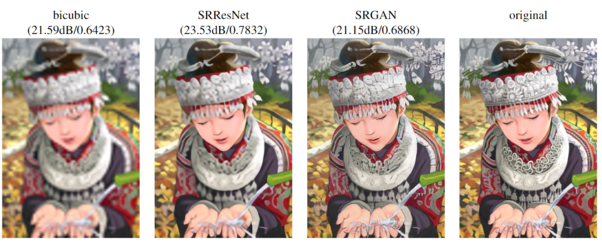
\includegraphics[scale=0.4]{sr}
% 	\caption{Example of the super-resolved images with $4 \times$ upscale factor, from left to right: bicubic interpolation, SRResNet, SRGAN, original HR image \cite{srgan_2016}.}
% 	\label{fig:sr}
% \end{figure}

\begin{figure}[b]
	\centering
	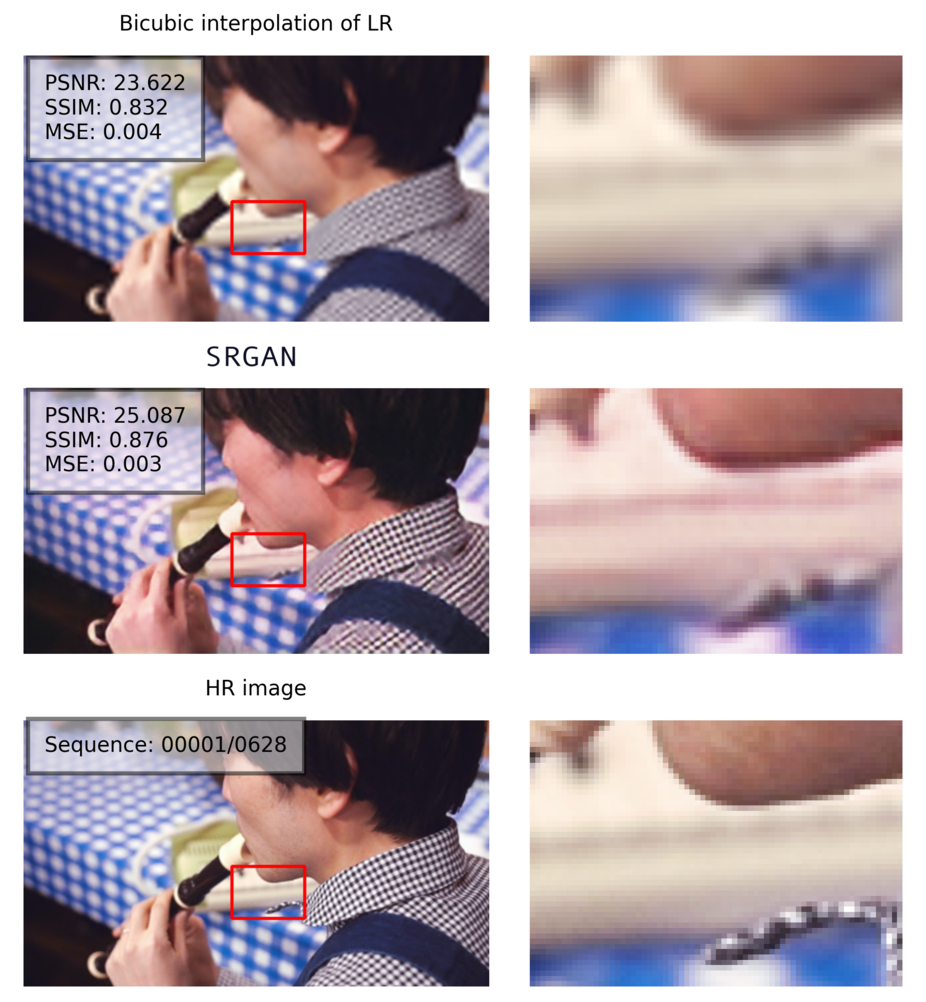
\includegraphics[scale=1.5]{results/crop_00001_0628}
	\caption{Example of the super-resolved frame generated using the SRGAN model (sequence 00001/0628 from Vimeo90K dataset)}
	\label{fig:example_sr_conclusion}
\end{figure}

Video plays an important role in our daily lives, making the enhancement of low-resolution videos through \acrshort{sr} techniques a crucial endeavor. Video super-resolution originates from image super-resolution and has the objective of enhancing the quality of high-resolution videos by reconstructing them from several low-resolution frames. Nevertheless, it is crucial to note that video super-resolution differs notably from image super-resolution since it typically utilizes inter-frame data to achieve its results.

The progress in computing power and deep learning approaches has sparked a multitude of advancements in video-related problems, including frames interpolation, artifact removal, denoising, deblurring, and super-resolution. In this thesis, we focus on \acrshort{vsr} problem applying \acrshort{gan} based approach that is a rapidly developing field.

Over the past few years, there has been a consistent increase in the resolution of consumer devices, including monitors, displays, virtual reality headsets, and other similar technologies. Content that was created in the past may not appear optimal on high-resolution screens for the users. Possibility of real-time \acrshort{vsr} techniques could have significant implications for the entertainment industry, particularly in the context of streaming services. As the demand for streaming platforms continues to soar, applying post-processing VSR approaches on the client side can be feasible, thereby reducing the requirement for large-scale data transfers \cite{video_super_resolution_survey_2020}.

In this work, we investigate existing \acrshort{vsr} approaches based on \acrshortpl{gan} and selected the SRGAN \cite{srgan_2016} model for the research. We study whether \acrlong{sisr} methods based on \acrshortpl{gan} can be applied to \acrlong{vsr} problem and if it can achieve super-resolution performance comparable to \acrshort{vsr} models. We trained several SRGAN models with different parameters on Vimeo90K dataset, see an example of the super-resolved video frame on Fig. \ref{fig:example_sr_conclusion}.

First, we study if the SRGAN model can be used to the \acrshort{vsr} problem and to what temporal inconsistencies and artifacts it can lead. Second, the loss function components are analyzed with emphasis on the total-variation loss. At last, we study the effect of different patch size values on the model's training and performance.

% Three paragraphs defining your field, importance of your topic and why it is significant to work on it today.

% One paragraph defining the work that has been done in this field, with a table summarizing the work that has been done in literature.

% One paragraph defining what has not been done (Gap analysis).

% One paragraph on what you are doing in this work (one main and at least two smaller research questions) and your contribution/novelty of your work.

% One paragraph concluding the introduction section with an overall summary of methods, results, and discussion.

\section{Literature Review}
Three - four paragraphs (or more) with one paragraph per important literature.
A table summarizing the characteristics of the existing literature along with the novelty of your proposed work (as shown in Table~\ref{tab:LiteratureSummary}).

\subsection{Generative Adversarial Networks}

\Acrfullpl{gan} belong to the class of generative models used in unsupervised machine learning. They consist of two networks, namely the generator and the discriminator, engaged in a competitive zero-sum game framework. \Acrshortpl{gan} employ a latent code that encapsulates all aspects of the generated output.

In the \acrshort{gan} framework, we have two models engaged in a competitive scenario akin to game theory. The setup involves a game with defined payoff functions, where each player strives to maximize their respective payoffs. In this game, one of the networks serves as the generator, which is our main focus and is responsible for producing samples (also known as generated or fake samples) with the goal of imitating those originating from the real training distribution (real samples). The other competing model is the discriminator, which examines the samples and determines whether they are real or fake \cite{gans_overview_2018}.

During training, images or other samples are provided to the discriminator. The discriminator is typically a differentiable function, often implemented as a deep neural network, whose parameters can be learned through gradient descent. When the discriminator is presented with samples/images from the training set (real samples), its objective is to output a value close to one, indicating a high probability that the input is real rather than fake \cite{gans_overview_2018}.

The discriminator is also used to evaluate samples generated by the generator (fake samples), and in this case, the objective of the discriminator is to produce an output as close to zero as possible, indicating that the sample is fake. The generator, on the other hand, is a differentiable function, often implemented as a deep neural network, and its parameters can be learned through gradient descent \cite{gans_overview_2018}.

The generator function operates on a sampled latent vector 'z', which serves as initial noise and acts as a source of randomness to aid the generator in producing a diverse range of outputs. The images generated by the generator are then evaluated by the discriminator, and the generator strives to trick the discriminator into outputting a value of one, making it believe that the generated image is real when, in fact, it is not. For more detailed technical information on \acrshortpl{gan}, readers can refer to \cite{gans_overview_2018}.




\subsection{Video Super-Resolution Overview}

Over the past few years, numerous video super-resolution techniques have emerged, dividing mainly into two categories: traditional approaches and deep learning-based approaches. Traditional super-resolution methods are categorized into three groups: interpolation-based, reconstruction-based, and frequency-based approaches.

So far, many \acrshort{vsr} algorithms have been proposed. Different deep learning models have demonstrated their effectiveness in video super-resolution tasks. Video Super-Resolution typically adopts the multi-input-single-output approach, as it involves providing multiple low-resolution frames to the model to predict a single reference frame. The key emphasis in VSR is on capturing the spatial and temporal relationships between frames.

In Liu et al. \cite{video_super_resolution_survey_2020} the existing VSR methods are categorized into two main categories: methods with alignment and methods without alignment, according to whether the video frames are explicitly aligned.

\begin{figure}[t]
    \centering
    % 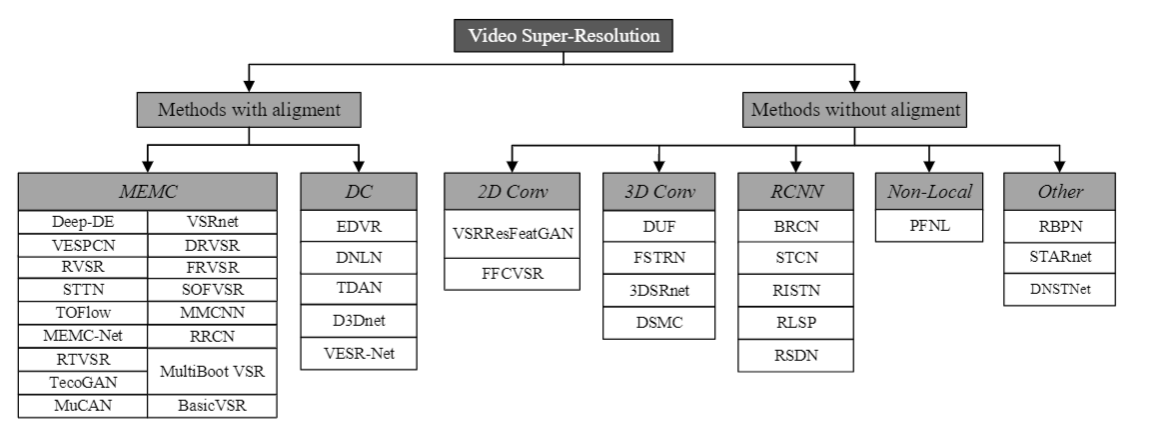
\includegraphics[scale=1]{vsr_methods}
    \centerline{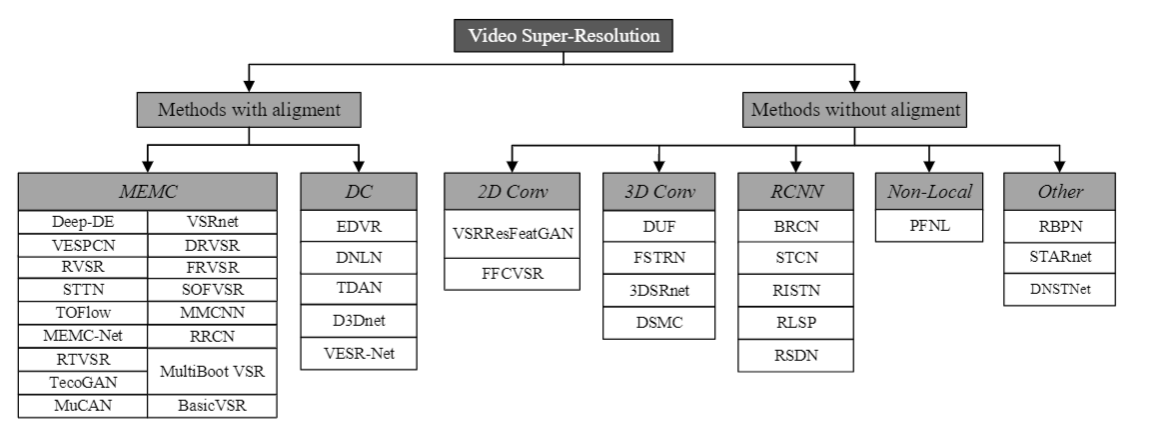
\includegraphics[width=8.9cm]{vsr_methods}}
    \caption{A classification scheme for the current state-of-the-art video super-resolution methods \cite{video_super_resolution_survey_2020}}
    \label{fig:vsr_methods}
\end{figure}

A classification of the current \acrshort{vsr} methods is presented at Fig. \ref{fig:vsr_methods}. There, MEMC stands for Motion Estimation and Compensation, DC is Deformable Convolution, 3D Conv means 3D Convolution and RCNN is Recurrent Convolutional Neural Network \cite{video_super_resolution_survey_2020}.

\subsection{Frame-Reccurent Video Super-Resolution}

Frame recurrent video super-resolution (FRVSR), as proposed by Sajjadi et al. \cite{frvsr_2018}, focuses on using the previously inferred high-resolution (HR) estimate to super-resolve the subsequent frame. This approach aims to achieve temporally consistent results and reduce computational costs. The architecture of FRVSR is presented in Figure \ref{frvsr_arch}.

\begin{figure}[htb]
    \centering
    \centerline{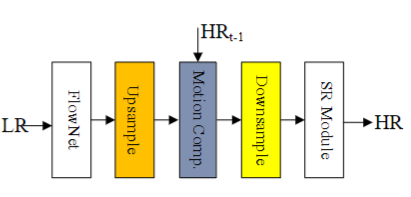
\includegraphics[width=8.9cm]{frvsr_arch}}
    \caption{The network architecture of FRVSR \cite{video_super_resolution_survey_2020}}
    \label{fig:frvsr_arch}
\end{figure}

The detailed implementation involves the use of an optical estimation network to compute the optical flow between the previous frame and the target frame. Subsequently, the low-resolution optical flow is upsampled to match the size of the high-resolution video using bilinear interpolation. The HR variant of the previous frame is then warped using the upsampled LR optical flow, and the warped HR frame is downsampled using space-to-depth transformation to obtain the LR version. Finally, the LR variant of the warped HR frame and the target frame are fed into the subsequent super-resolution network to produce the result for the target frame \cite{video_super_resolution_survey_2020}.

\subsection{TecoGAN}

The Temporally coherent GAN (TecoGAN) by Chu et al. \cite{tecogan_2018} introduces a spatio-temporal discriminator to achieve realistic and coherent video super-resolution. To address recurrent artifacts, they propose a new "Ping-Pong" loss. Similar to GANs, TecoGAN comprises a generator and a discriminator, and its architecture is illustrated in Fig. \ref{fig:tecogan}.

\begin{figure}[htb]
    \centering
    \centerline{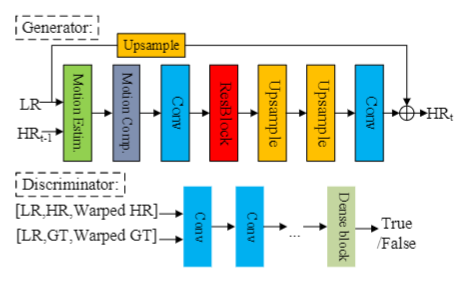
\includegraphics[width=8.9cm]{tecogan}}
    \caption{The network architecture of TecoGAN \cite{video_super_resolution_survey_2020}}
    \label{fig:tecogan}
\end{figure}

\subsection{VSRResFeatGAN}

Rather than employing alignment operations like motion estimation and motion compensation between frames, the input frames are directly fed into a 2D convolutional network for spatial feature extraction, fusion, and super-resolution operations. This approach simplifies the video super-resolution problem by allowing the network to independently learn the correlation information within frames. Representative methods following this approach include VSRResFeatGAN (Lucas et al. \cite{GANs_perc_loss_vsr_2018}) and FFCVSR (Yan et al. \cite{Yan_frame_vsr_2019}).

\subsection{iSeeBetter}

iSeeBetter \cite{iSeeBetter_2020} is a GAN-based spatio-temporal method used for video super-resolution that renders temporally consistent super-resolution videos. iSeeBetter's generator utilizes recurrent back-projection networks to extract spatial and temporal information from both the current and neighboring frames. To enhance the natural appearance of the super-resolved image and eliminate artifacts associated with conventional methods, they incorporate the discriminator from the super-resolution generative adversarial network (SRGAN).

\subsection{Loss function\label{sec:loss_function}}

\begin{figure}[!htb]
	\centering
    \centerline{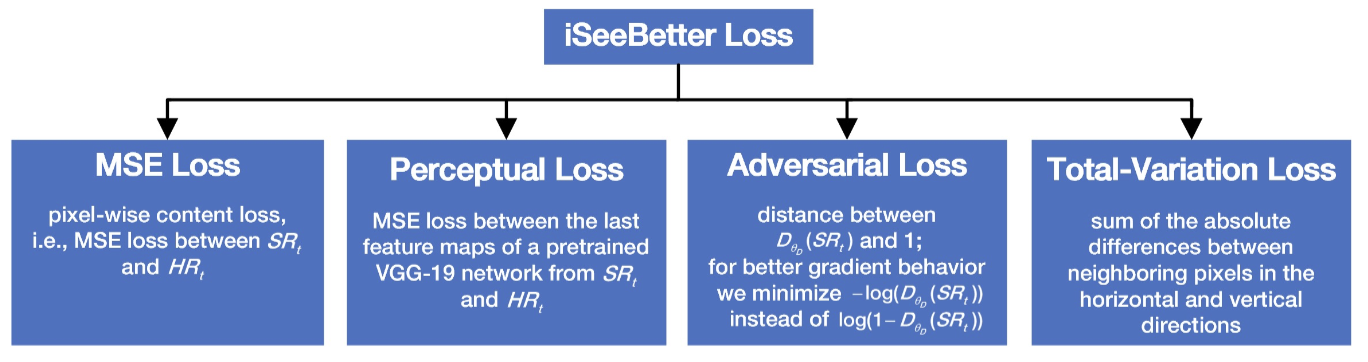
\includegraphics[width=8.9cm]{loss}}
	\caption{The \acrshort{mse}, perceptual, adversarial and \acrshort{tv} loss components \cite{iSeeBetter_2020}.}
	\label{fig:loss}
\end{figure}

The perceptual image quality of the resulting SR image is dependent on the choice of the loss function. To evaluate the quality of an image, MSE is the most commonly used loss function in a wide variety of state-of-the-art SR approaches, which aims to improve the \acrshort{psnr} of an image. Despite optimizing \acrshort{mse} makes better \acrshort{psnr} and \acrshort{ssim} numbers, these metrics does not take into account fine details in the image, potentially misrepresenting the perceptual quality \cite{iSeeBetter_2020}. \acrshort{mse}'s capability to capture intricate texture details by analyzing individual pixel differences in consecutive frames is highly restricted, leading to the potentially excessively smooth video frames \cite{fast_video_super_reso_ann_2012}. Through a sequence of experiments, it was discovered that even when images were deliberately distorted manually, their \acrshort{mse} scores were similar to those of the original, undistorted image \cite{universal_image_quality_index_2002}.

To address this, \cite{iSeeBetter_2020} uses a four-fold (\acrlong{mse}, perceptual, adversarial, and \acrlong{tv}) loss instead of solely relying on pixel-wise \acrshort{mse} loss. Fig. \ref{fig:loss} shows the components of the loss function used in this work.

\subsubsection{Mean-Squared Error Loss}

In this work we use \acrshort{mse} loss (or, alternatively, content loss) for the super-resolved frame $I^{SR}$ against the ground truth $I^{HR}$:

\begin{equation} \label{eq:mse_loss}
	L_{MSE} = \frac{1}{WH} \sum_{x=0}^{W} \sum_{y=0}^{H} ( I^{HR}_{x,y} - G_{\theta_G} (I^{LR})_{x,y} )^2
\end{equation}

where, $G_{\theta_G} (I^{LR})$ is the estimated frame SR, $W$ and $H$ are width and height of the image frames correspondingly \cite{iSeeBetter_2020}.

\subsubsection{Perceptual Loss \label{sec:perceptual_loss}}

Instead of utilizing low-level measures that focus on pixel-wise errors, perceptual loss relies on features extracted from the activation layers of the pre-trained VGG network in the reference paper \cite{vgg_very_deep_cnn_2014}. Perceptual loss, which was introduced in \cite{sr_with_deep_conv_sufficient_stats_2015, texture_synth_cnn_2015}, focuses on perceptual similarity instead of similarity in pixel space.

Here perceptual loss is defined the Euclidean distance between the feature representations of the estimated SR image $G_{\theta_G} (I^{LR})$ and the ground truth image $I^{HR}$:

\begin{gather*} %\label{eq:perceptual_loss}
	L_{perceptual} = \frac{1}{W_{i,j} H_{i,j}} \sum_{x=0}^{W_{i,j}} \sum_{y=0}^{H_{i,j}} ( VGG_{i,j} (I^{HR}_{x,y}) \\- VGG_{i,j} (G_{\theta_G} (I^{LR})_{x,y}) )^2
\end{gather*}

where, $VGG_{i,j}$ is the feature map which is the result of the $j^{th}$ convolution after activation before the maxpooling layer in the VGG network, $W_{i,j}$ and $H_{i,j}$  are the widths and heights of the corresponding feature maps in VGG model \cite{iSeeBetter_2020}.

\subsubsection{Adversarial Loss\label{sec:adversarial_loss}}

Adversarial loss is defined as:

\begin{equation} \label{eq:adversarial_loss}
	L_{adversarial} = -\log ( D_{\theta_D}( G_{\theta_G} (I^{LR}) ) )
\end{equation}

where $D_{\theta_D}$ is the output of the discriminator which is the probability that the reconstructed image $G_{\theta_G} (I^{LR}$ is a real HR image. It was shown in \cite{goodfellow2014generative} that it is better for the gradient behavior to minimize $-\log ( D_{\theta_D}( G_{\theta_G} (I^{LR}) ) )$ instead of $\log (1 - D_{\theta_D}( G_{\theta_G} (I^{LR}) ) )$

\subsubsection{Total-Variation Loss\label{sec:total_variation_loss}}

\acrshort{tv} loss was proposed in \cite{image_upsampling_total_variation_regularization_2005} as a loss function for super-resolution problems. It is defined as the sum of the absolute differences between neighboring pixels in the horizontal and vertical directions. By incorporating TV loss into our overall loss objective, we aim to minimize noise in the input, leading to a denoised output super-resolution image that promotes spatial smoothness.

\acrshort{tv} loss is defined as in \cite{deep_learning_image_sr_2020}:

\begin{gather*} \label{eq:tv_loss}
	L_{TV} = \frac{1}{WH} \sum_{x=0}^{W} \sum_{y=0}^{H}  ((G_{\theta_G} (I^{LR})_{i, j+1} - G_{\theta_G} (I^{LR})_{i, j})^2 + \\(G_{\theta_G} (I^{LR})_{i+1, j} - G_{\theta_G} (I^{LR})_{i, j})^2 )^{\frac{1}{2}}
\end{gather*}

\subsubsection{Loss formulation}

The overall loss objective for each frame is defined as a combination of the MSE, adversarial, perceptual, and TV loss components, with appropriate weights assigned to each component:

\begin{equation} \label{eq:total_Gloss}
	\begin{split}
		L_{G_{\theta_G}} &= \alpha \times L_{MSE}(I^{SR}, I^{HR}) + \\
		& \beta \times L_{perceptual} (I^{SR}, I^{HR}) + \\
		& \gamma \times L_{adversarial}  + \\
		& \delta \times L_{TV} (I^{SR}, I^{HR})
	\end{split}
\end{equation}

where $\alpha, \beta, \gamma, \delta$ are weights.

\subsection{TV loss weight}

\Acrfull{tv} denoising technique is known in image processing \cite{nonlinear_total_variation_noise_removal_1992}. The \acrlong{tv} based loss component was introduced in the original SRGAN paper \cite{srgan_2016} for training of SRResNet-VGG22 model. The \acrshort{tv} loss weight was set to $2 \times 10^{-8}$. The same value of \acrshort{tv} loss $\delta=2 \times 10^{-8}$ is used in \cite{iSeeBetter_2020} and \cite{iSeeBetter_milestone}.

The effect of \acrshort{tv} loss on the performance of the SRGAN model for the face \acrlong{sr} was studied in \cite{SRGAN_with_tv_loss_face_2020} where the \acrshort{tv} loss weight was also set to $2 \times 10^{-8}$ with reference to the SRGAN implementation by Hao Ren \footnote{Github page: https://github.com/leftthomas/SRGAN}.

\Acrshort{tv} loss was used in the research related to the style transfer and \acrlong{sr} \cite{Perceptual_Losses_for_Real_Time_Style_Transfer_and_Super_Resolution_2016} where they set \acrlong{tv} regularization "with a strength of between $1 \times 10^{-6}$ and $1 \times 10^{-8}$, chosen via cross-validation per style target" \cite{Perceptual_Losses_for_Real_Time_Style_Transfer_and_Super_Resolution_2016}.

Following an extensive literature review, we encountered a lack of sufficient explanation for the selected \acrshort{tv} loss weight values utilized in the aforementioned research works. Consequently, we aim to conduct an in-depth investigation into this topic to offer more profound insights into the optimal range of \acrshort{tv} loss weight values for the SRGAN model in the context of the \acrshort{vsr} problem. The summarized review of different \acrshort{tv} vaues is shown in Table \ref{tab:tv_loss_summary}.

\begin{table*}[!tb]
\centering
\caption{Literature review table showing the contributions of various authors for quantization of networks.}
\label{tab:tv_loss_summary} 
	\begin{tabular}{|l|c|l|}
	\hline
	  \thead{Paper}                                                     & \thead{TV loss\\weight}       & \thead{Reasoning}                                      \\ \hline
    SRGAN paper \cite{srgan_2016}                             & $2 \times 10^{-8}$   & References to \cite{image_upsampling_total_variation_regularization_2005}, \cite{Perceptual_Losses_for_Real_Time_Style_Transfer_and_Super_Resolution_2016} \\ \hline
	  Faces SR paper  \cite{SRGAN_with_tv_loss_face_2020} & $2 \times 10^{-8}$ & \makecell{Reference to implementation\\(based on \cite{srgan_2016})}  \\ \hline
	  Style transfer paper  \cite{Perceptual_Losses_for_Real_Time_Style_Transfer_and_Super_Resolution_2016} & $10^{-6} - 10^{-8}$  & \makecell{"chosen via cross-validation\\per style target"} \\ \hline
	  iSeeBetter paper \cite{iSeeBetter_2020}              & $2 \times 10^{-8}$        & References to \cite{HandsOn_GANs_2019}                \\ \hline
	  iSeeBetter milestone paper \cite{iSeeBetter_milestone} & $2 \times 10^{-8}$        & References to \cite{single_vsr_gan_pseudo_inverse_2019}                \\ \hline
\end{tabular}
\end{table*}


\section{Methodology}
\subsection{Dataset}

To train the model in this thesis, we use a subset of the original test set of Vimeo90K dataset (not downsampled or downgraded by noise, \(\sim \)15GB of video frames) \cite{vimeo90k_2019}. The septuplet dataset consists of 91,701 7-frame sequences with fixed resolution $448 \times 256$, extracted from 39K selected video clips from Vimeo-90K. This dataset is designed to video denoising, deblocking, and super-resolution. Apart from Vimeo90K dataset, we use other datasets, that are known in the \acrlong{sr} research, for the evaluation of the trained models and comparison of our results with other authors.

\begin{table*}[!htb]
    \centering
    \caption{Datasets summary.}
    \label{tab:datasets}
	\begin{tabular}{|l|c|c|c|c|}
	\hline
	Dataset  & Amount & \makecell{Average\\resolution} & Format & Keywords  \\ \hline
	Set5     & 5      & $313 \times 336$   & PNG    & baby, bird, butterfly, head, woman \\ \hline
	Set14    & 14     & $492 \times 446$   & PNG    & humans, animals, insects, etc. \\ \hline
	Urban100 & 100    & $984 \times 797$   & PNG    & architecture, city, structure, urban, etc. \\ \hline
	BSD100   & 100    & $435 \times 367$   & PNG    & animal, building, food, etc. \\ \hline
	Vid4     & 171    & $720 \times 480$   & PNG    &  calendar, city, foliage, walk \\ \hline
\end{tabular}
\end{table*}

\section{SRGAN model architecture\label{sec:srgan_arhitecture}}

\begin{figure}[!htb]
	\centering
	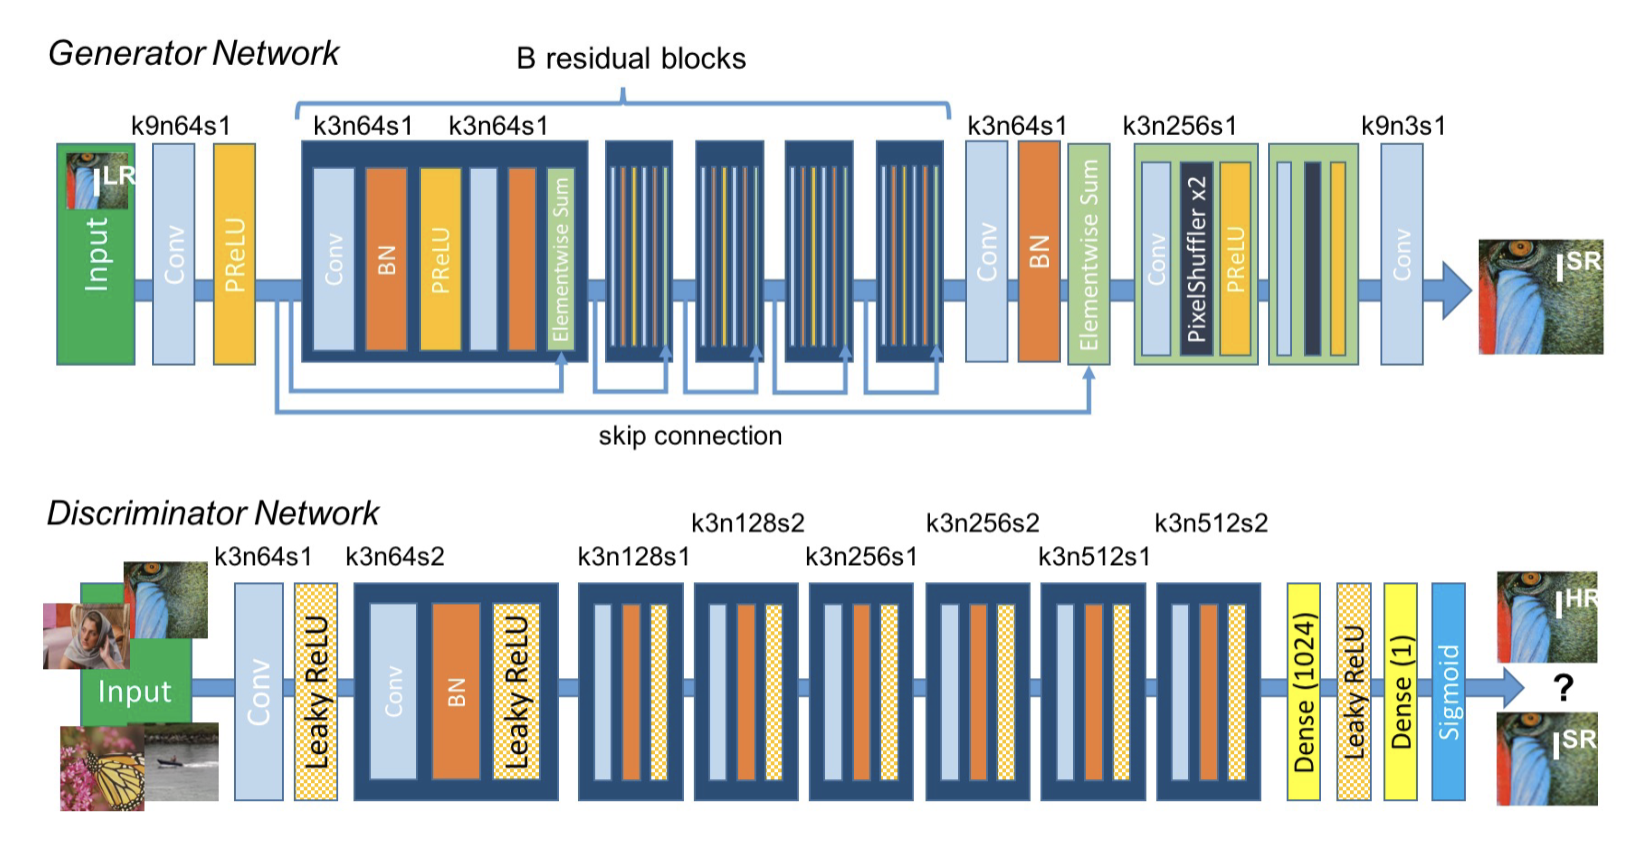
\includegraphics[scale=0.5]{srgan_model}\\
	\caption{Architecture of Generator and Discriminator Network. Here $k$ is the corresponding kernel size, $n$ is a number of feature maps and $s$ is stride indicated for each convolutional layer.}
	\label{fig:srgan_model}
\end{figure}

\acrshortpl{gan} offer a robust framework for generating visually convincing natural images that possess a high level of perceptual quality. The \acrshort{gan} process encourages the generated images to transition towards areas in the solution space that are more likely to contain photo-realistic images. As a result, the generated images become closer to the manifold of natural images, capturing their characteristics and visual realism \cite{goodfellow2014generative}.

We define a discriminator network $D_{\theta_D}$ optimized together with $G_{\theta_G}$ to solve the adversarial min-max problem:

\begin{gather*} \label{eq:adversarial_min_max}
	\min_{\theta_G} \max_{\theta_D} \mathbb{E}_{I^{HR} \sim p_{train} (I^{HR}) }  [ \log D_{\theta_D}(I^{HR})  ] + \\
	\mathbb{E}_{I^{LR} \sim p_G (I^{LR})} [ \log (1 - D_{\theta_D} ( G_{\theta_G} (I_{LR}) )) ]
\end{gather*}

The main concept behind this formulation is to enable the training of a generative model $G$. The objective is to deceive a differentiable discriminator $D$, which is specifically trained to differentiate between super-resolved images and real images. By adopting this approach, the generator network can acquire the ability to generate solutions that closely resemble real images, making them challenging for the discriminator to classify accurately. This strategy promotes the generation of visually superior solutions that align with the characteristics of natural images. In contrast, conventional super-resolution solutions achieved by minimizing pixel-wise error measurements like \acrshort{mse} do not prioritize perceptual quality.

The architecture of the generator network is shown on Fig. \ref{fig:srgan_model}. It consists of $B$ residual blocks with the same layout of two convolutional layers with $3 \times 3$ kernels and 64 feature maps, batch-normalization layers and ParametricReLU \cite{delve_deep_into_rectifiers_2015} as the activation function. The resolution of the input image is increased by two trained sub-pixel convolution layers \cite{sub_pixel_cnn_2016}.

The discriminator network is trained to distinguish between the real HR images from generated SR images. The discriminator architecture is shown in Fig. \ref{fig:srgan_model}. The discriminator model is trained to solve the optimization problem in Equation \ref{eq:adversarial_min_max}. It contains eight convolutional layers with an increasing number of $3 \times 3$ filter kernels, increasing by a factor of 2 from 64 to 512 kernels as in the VGG network \cite{vgg_very_deep_cnn_2014}. Strided convolutions are employed to decrease the image resolution each time the number of features is doubled. After the resulting 512 feature maps there are two dense layers and a final sigmoid activation function to produce a probability for sample classification \cite{srgan_2016}.

\subsection{Detailed Methodology}
Three paragraphs for explaining the pipeline and workflow of your study.
A figure depicting the workflow of your work (shown in Fig~\ref{Fig:Figure1} or in Fig~\ref{Fig:Figure3b}).

\begin{figure*}[htbp]
\centerline{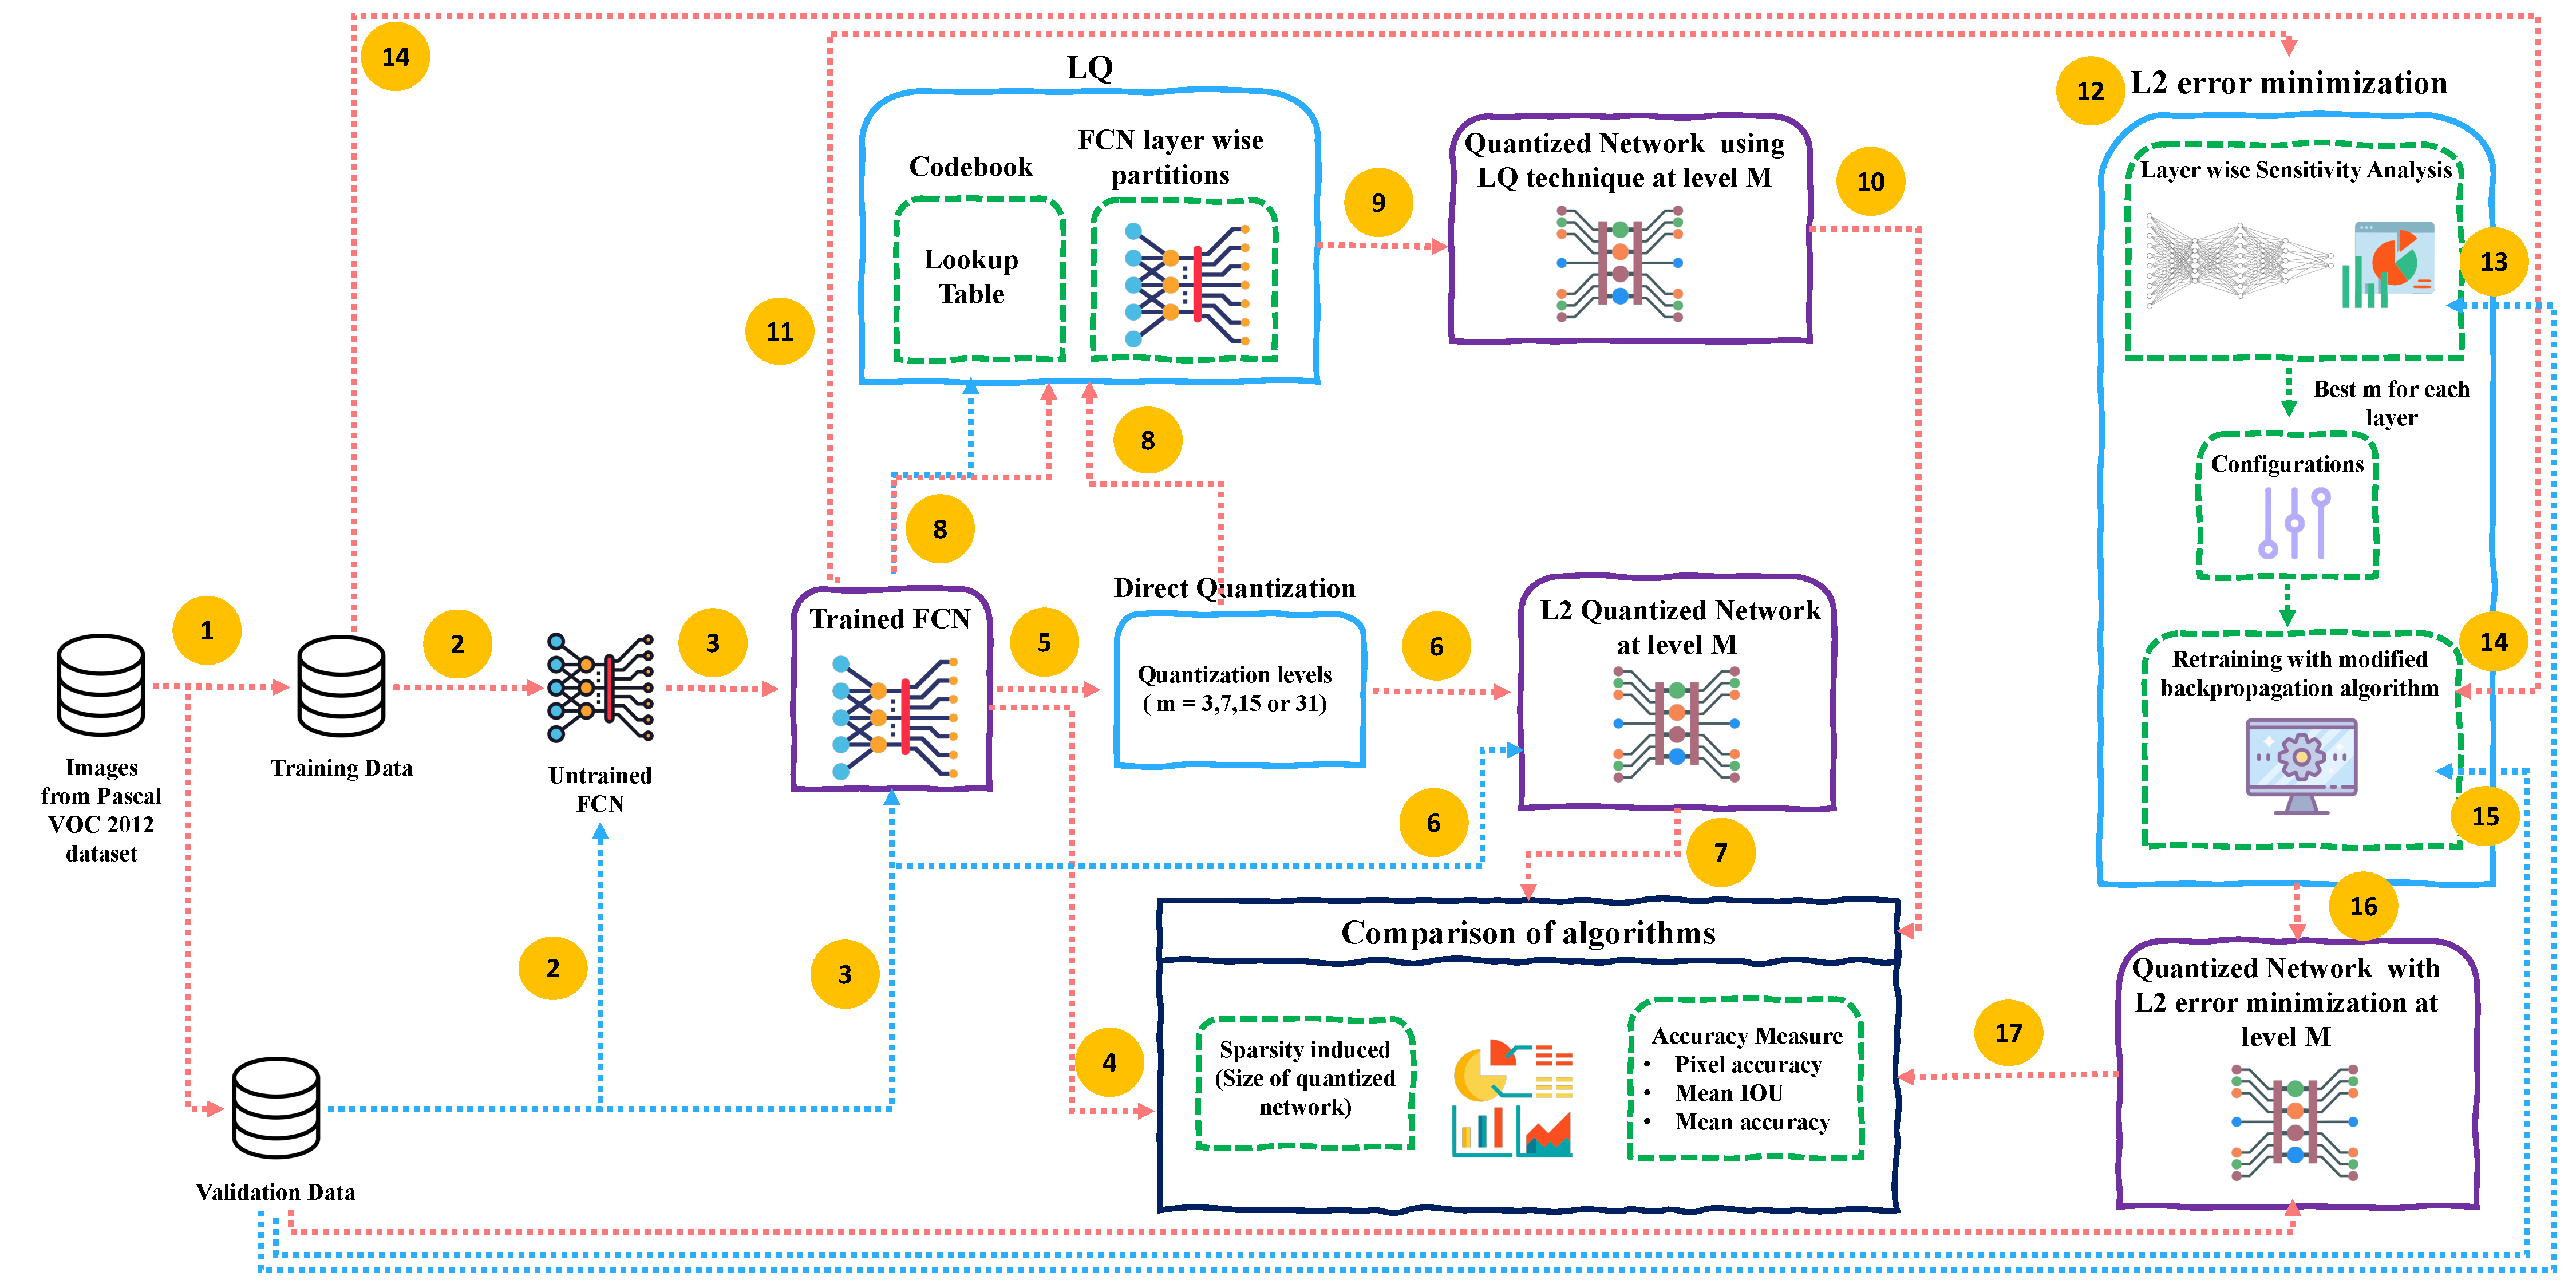
\includegraphics[width=17.8cm]{Figure1.pdf}}
\caption{Sample workflow image. Make it in Powerpoint with svg images and save as pdf. Sanity check: Zoom in and pixels should not break.}
\label{Fig:Figure1}
\end{figure*}

\begin{figure*}[htbp]
\centerline{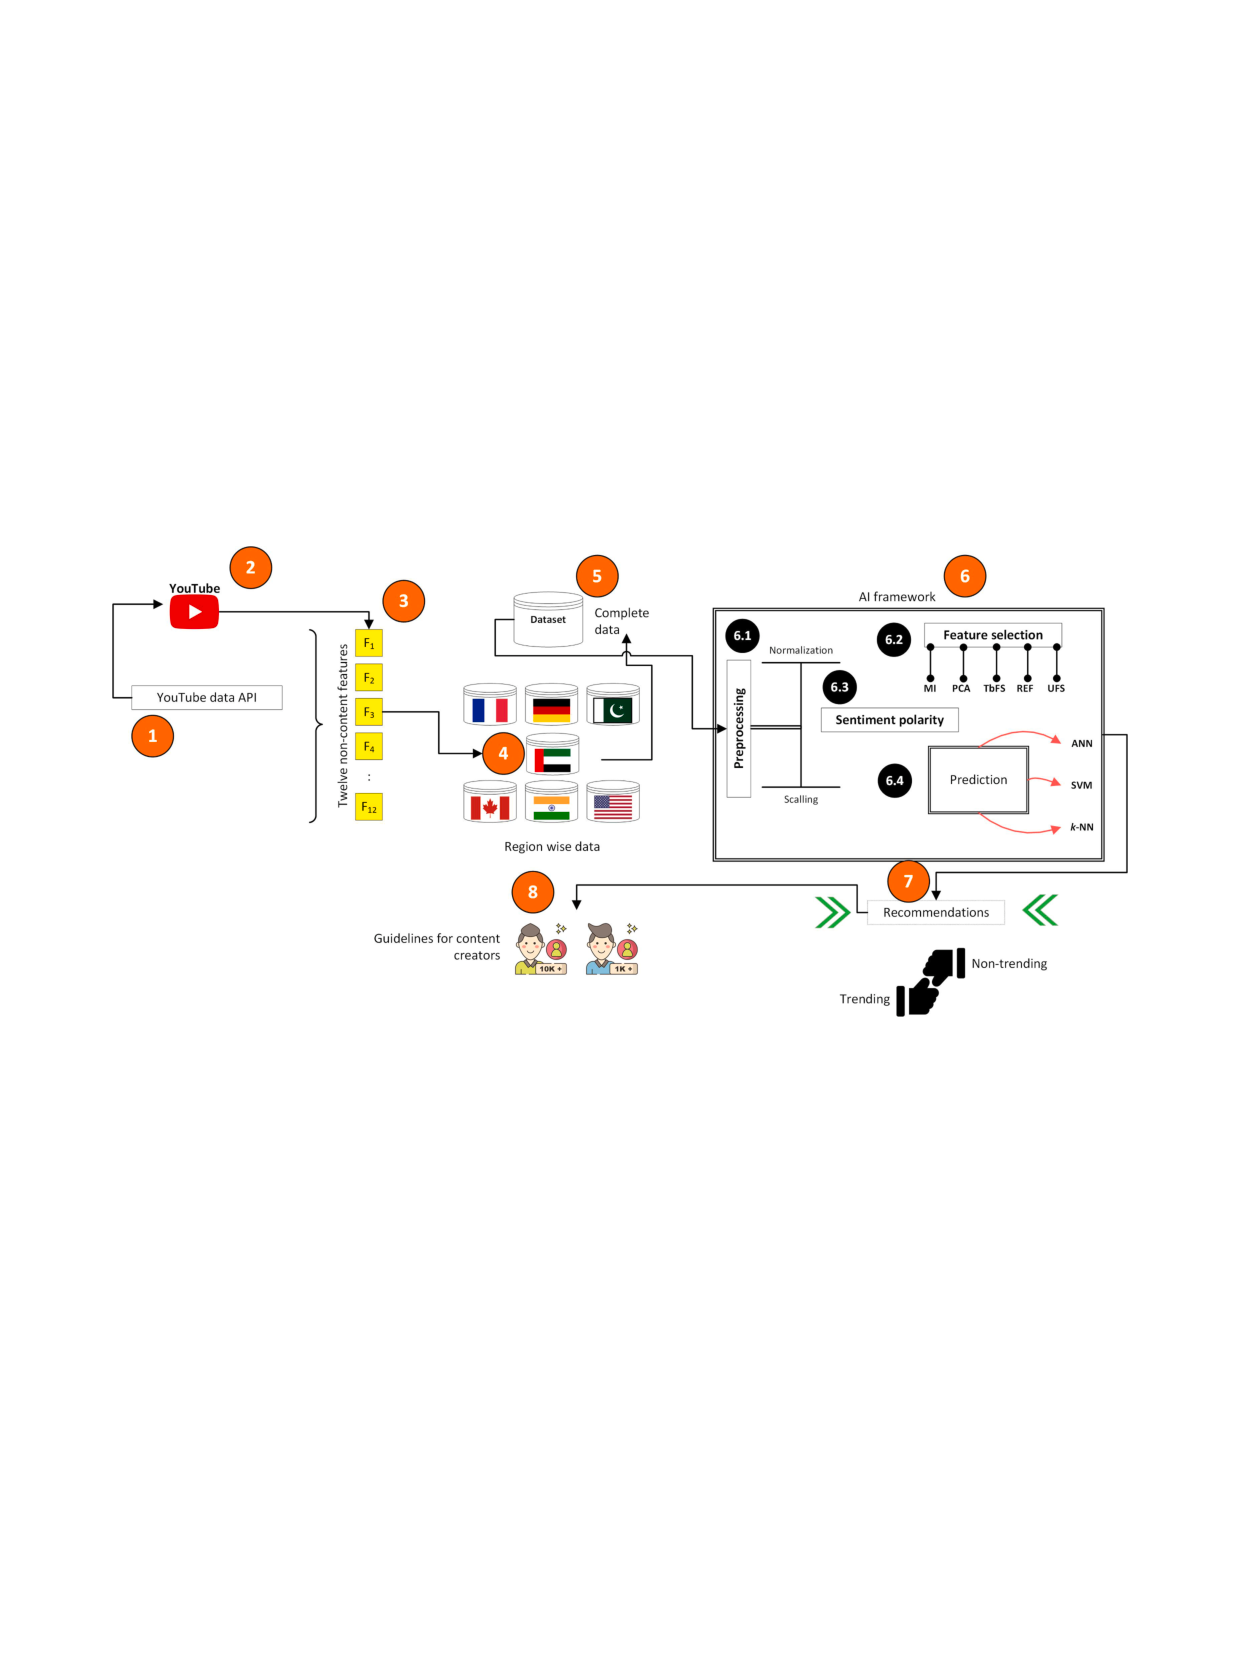
\includegraphics[width=17.8cm]{Figure3b.pdf}}
\caption{Sample workflow image. Make it in Powerpoint with svg images and save as pdf. Sanity check: Zoom in and pixels should not break.}
\label{Fig:Figure3b}
\end{figure*}

\subsection{Evaluation Metrics}
Video quality refers to the visual attributes of videos, which can be evaluated using either quantitative metrics or perceptual assessments conducted by human viewers. While human assessments offer initial insights, quantitative metrics are essential for benchmarking results and gaining widespread acceptance within the scientific community. This study primarily concentrates on achieving results based on reconstruction accuracy and perceptual naturalness, thereby considering metrics such as \acrfull{mse}, \acrfull{psnr}, and \acrfull{ssim}. These metrics are classified as full-reference metrics, meaning they require both the target (original) and the reconstructed (super-resolved) output to calculate the image/video quality \cite{deep_learning_image_sr_2020}.

\subsubsection{Mean Squared Error}

One widely-used metric is \acrfull{mse}, which is defined by the Equation \ref{eq:mse_metric}:

\begin{equation} \label{eq:mse_metric}
    MSE = \frac{1}{N} \sum_{i}^{N} (\hat{I}_i - \tilde{I}_i)^2
\end{equation}

where $N$ is the total number of pixels in the frame, $\hat{I}$ is the ground-truth HR image, and $\tilde{I}$ is the super-resolved frame.

\subsubsection{Peak Signal to Noise Ratio}

\Acrfull{psnr} is one of the most popular reconstruction quality measurement of lossy transformation such as image compression. For image
super-resolution, PSNR is defined via the maximum pixel value and the \acrshort{mse} between images. \Acrshort{psnr} of one \acrshort{sr} frame is defined as \cite{video_super_resolution_survey_2020}:

\begin{equation}  \label{eq:psnr_metric}
    PSNR = 10 \log_{10} (\frac{L^2}{MSE})
\end{equation}

where $L$ is the maximum range of the pixel color value (usually 255). In general, a higher value of PSNR means superior quality of the image. Because \acrshort{psnr} relies solely on pixel-level \acrshort{mse}, it focuses solely on pixel differences without considering visual perception. Consequently, it often yields unsatisfactory results in representing the true reconstruction quality in real-world scenarios, where human perception matters more. Nevertheless, as a necessity to compare with existing literature and due to the absence of entirely accurate perceptual metrics, PSNR remains the most commonly used evaluation criterion for \acrshort{sr} models \cite{deep_learning_image_sr_2020}.

\subsubsection{Structural Similarity Index Metric}

The \acrfull{ssim} is defined for measuring the structural similarity between images, based on independent comparisons of luminance, contrast, and structures \cite{ssim_2004}. For an image $I$ with $N$ pixels, the luminance $\mu_I = \frac{1}{N} \sum_{i=1}^{N} I(i)$ and contrast $\sigma_I = (\frac{1}{N-1} \sum_{i=1}^{N} (I(i) - \mu_I)^2)^{\frac{1}{2}}$ are calculated as the mean and standard deviation of the image intensity $I$.

The comparisons of luminance and contrast are denoted as $C_l(I, \hat{I})$ and $C_c(I, \hat{I})$ correspondingly, are defined by:

\begin{equation}  \label{eq:comp_luminosity}
    C_l(I, \hat{I}) = \frac{2 \mu_I \mu_{\hat{I}} + C_1 }{\mu_I^2 + \mu_{\hat{I}}^2 + C_1}
\end{equation}

\begin{equation}  \label{eq:comp_contrast}
    C_c(I, \hat{I}) = \frac{2 \sigma_I \sigma_{\hat{I}} + C_2 }{\sigma_I^2 + \sigma_{\hat{I}}^2 + C_1}
\end{equation}

where $C_l = (k_1 L)^2$ and $C_2 = (k_2 L)^2$ are constants preventing instabilities, $k_1 << 1$ and $k_2 << 1$ \cite{deep_learning_image_sr_2020}.

\Acrfull{ssim} is defined as:

\begin{equation}  \label{eq:ssim}
    SSIM(I,\hat{I}) = [C_l(I, \hat{I})]^{\alpha} [C_c(I, \hat{I})]^{\beta} [C_s(I, \hat{I})]^{\gamma}
\end{equation}

where $\alpha$, $\beta$ and $\gamma$ are control parameters for relative importance, $C_s$ is the structure comparison function, defined by:

\begin{equation}  \label{eq:structure_comp_f}
    C_s(I, \hat{I}) = \frac{\sigma_{I\hat{I}}+C_3}{\sigma_I \sigma_{\hat{I}}+C_3}
\end{equation}

where $\sigma_{I, \hat{I}}$ is the covariance between $I$ and $\hat{I}$ and $C_3$ is a constant \cite{deep_learning_image_sr_2020}.

\Acrfull{ssim} is designed as an enhancement over conventional metrics like peak \acrshort{psnr} and \acrshort{mse}. Its purpose is to provide improved performance in assessing the similarity between images.

\subsection{Experimental settings}
One paragraph for experimental settings of your and competing methods (if any).
(Optional) One paragraph for hyper-parameter settings and network architecture 

A table with hyper-parameter settings (shown in Table~\ref{tab:FCNConfiguration}) and a figure for network architecture (shown in Fig~\ref{Fig:Figure2}).

\begin{table}[!t]
\centering
\caption{Configuration table showing the network configuration of FCN used in this study. The table shows the various configuration settings used for FCN8.}
\label{tab:FCNConfiguration} 
\begin{tabular}{|l|c|}
\hline
\multicolumn{2}{|c|}{\textbf{Network Configuration}} 
\\ \hline
Epochs & 50 \\
Learning rate & 0.0001 \\
Mini batch size & 20 \\ 
Optimizer & SGD \\
Momentum & 0.9 \\
Weight decay & 0.0002 \\
$L_2$ Regularization & None \\
Samples in training set & 8498 \\
Samples in validation set & 786 \\ \hline
\end{tabular}
\end{table}

\begin{figure*}[htbp]
\centerline{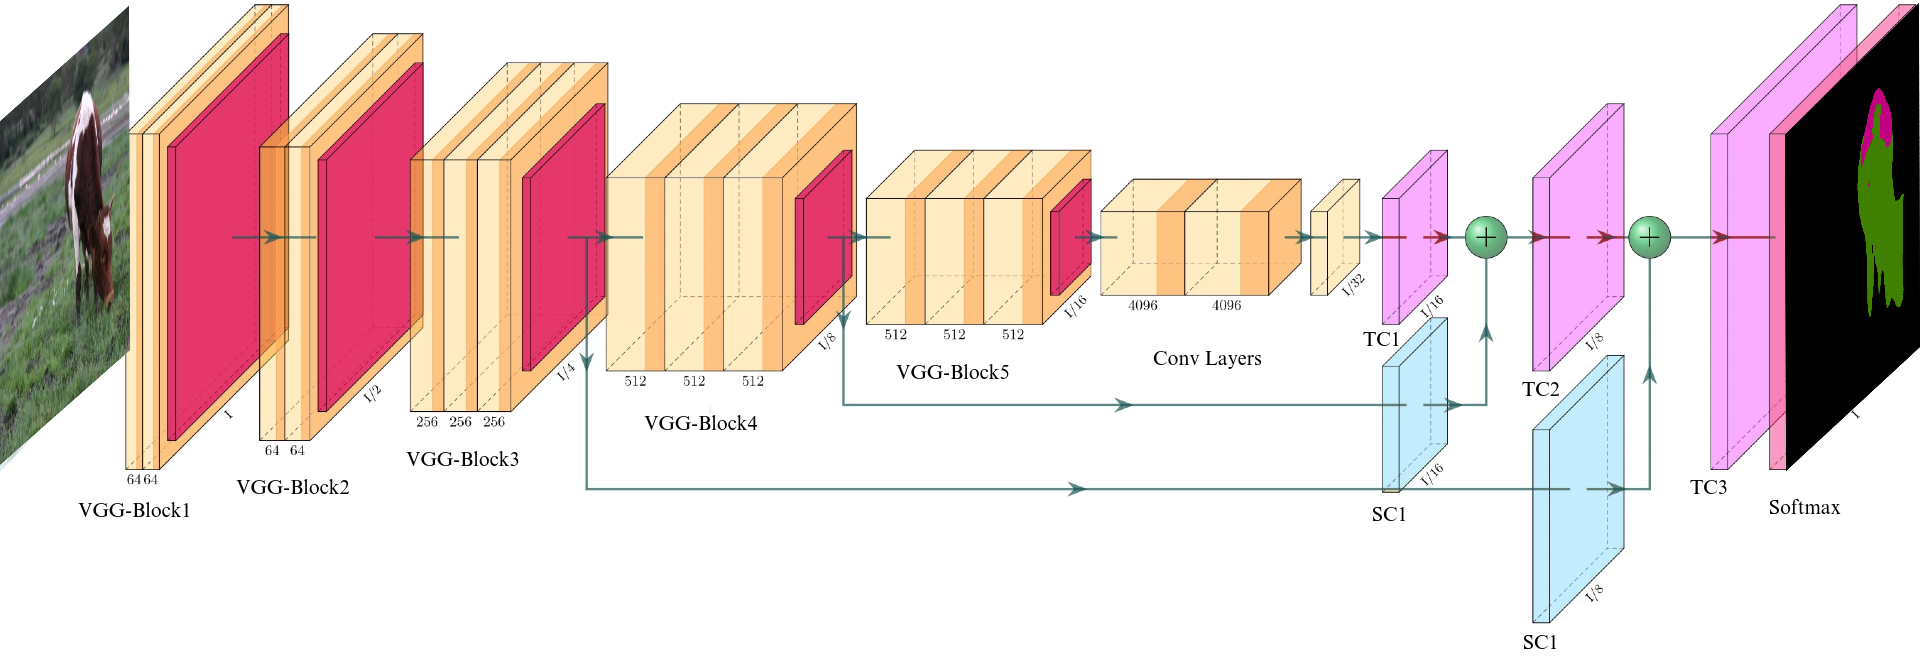
\includegraphics[width=17.8cm]{Figure2.png}}
\caption{Sample network architecture image. Make it in Powerpoint with svg images and save as pdf. Sanity check: Zoom in and pixels should not break.}
\label{Fig:Figure2}
\end{figure*}

\section{Results}
Three (or more) paragraph(s) explaining your results.~\cite{bayesian_vsr_2014}. 
At least one paragraph targeting one research question with at least one figure (preferably) or table (where figure is not possible).
Note that each figure must be drawn keeping in mind the black and white print (different patterns are prefered alongwith different intensity colors).
This section must contain only results and nothing else (not your own opinion or any sort of discussion on quality of results).
Also include comparison with existing contemporary methods in this section (sample shown in Figure~\ref{Fig:Figure4} and in Table~\ref{tab:LiteratureComparison}).

\begin{figure}[t!]
\centering
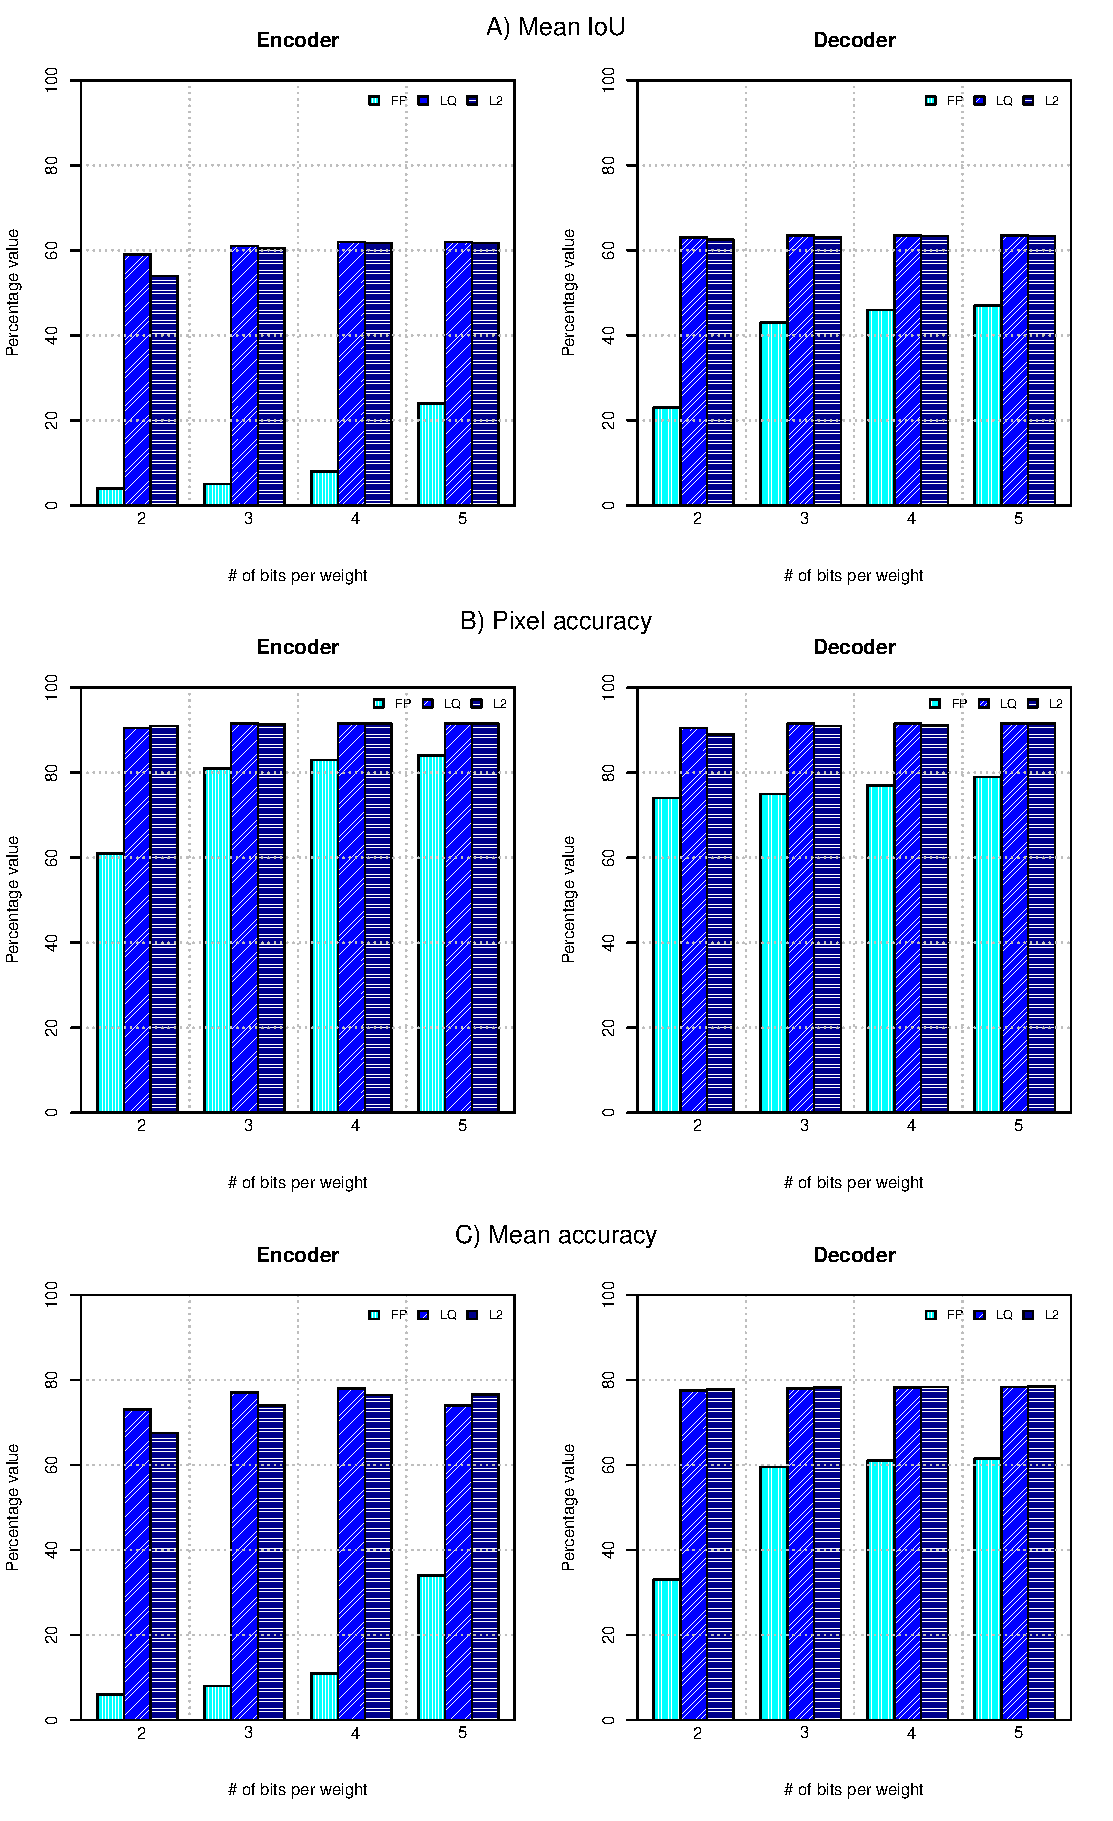
\includegraphics[width=8.9cm,keepaspectratio]{Figure4.pdf}
\caption{Sample Figure comparing the three quantization techniques Fixed Point (FP), Lloyd's quantizer (LQ) and $L_2$ error minimization ($L_2$) on the three performance metrics divided into encoder and decoder layers. Mean IoU is shown for the three techniques in Panel A), pixel accuracy in Panel B), and mean accuracy in Panel C) respectively. Note that FP is consistently worse than both LQ and $L_2$, while $L_2$ and LQ are of comparable accuracy. Also, FP is most sensitive to number of bits in all metrics while $L_2$ and LQ are relatively insensitive.}
\label{Fig:Figure4}
\end{figure}

\begin{table*}[!t]
\centering
\caption{Performance comparison table showing the performance of various quantization techniques applied on various networks. The results are directly taken from the papers after applying quantization on the mentioned datasets.}
\label{tab:LiteratureComparison} 
\begin{tabular}{|l|l|llllllll|}
\hline
\multirow{3}{*}{\begin{tabular}[c]{@{}l@{}}Paper \\ Name\end{tabular}} & \multicolumn{1}{c|}{\multirow{3}{*}{\begin{tabular}[c]{@{}c@{}}Dataset \\ Used\end{tabular}}}& \multicolumn{8}{c|}{Performance Comparison} \\ \cline{
3-10} 
 & \multicolumn{1}{c|}{}& \multicolumn{1}{c|}{\multirow{2}{*}{PA}} & \multicolumn{1}{c|}{\multirow{2}{*}{MA}} & \multicolumn{1}{c|}{\multirow{2}{*}{IoU}} & \multicolumn{1}{c|}{\multirow{2}{*}{Time}} & \multicolumn{1}{c|}{\multirow{2}{*}{\begin{tabular}[c]{@{}c@{}}Test \\ Error\end{tabular}}} & \multicolumn{1}{c|}{\multirow{2}{*}{\begin{tabular}[c]{@{}c@{}}Sparsity\\ Induced\end{tabular}}} & \multicolumn{1}{c|}{\multirow{2}{*}{\begin{tabular}[c]{@{}c@{}}size \\ reduction\end{tabular}}} & \multicolumn{1}{c|}{\multirow{2}{*}{\begin{tabular}[c]{@{}c@{}}memory \\ reduction\end{tabular}}} \\
 & \multicolumn{1}{c|}{}& \multicolumn{1}{c|}{}& \multicolumn{1}{c|}{}& \multicolumn{1}{c|}{} & \multicolumn{1}{c|}{}& \multicolumn{1}{c|}{} & \multicolumn{1}{c|}{}& \multicolumn{1}{c|}{} & \multicolumn{1}{c|}{} \\ \hline
\begin{tabular}[c]{@{}l@{}}Vanhoucke \\ et al. {[}26{]}\end{tabular} & $\times$& \multicolumn{1}{l|}{}& \multicolumn{1}{l|}{}& \multicolumn{1}{l|}{} & \multicolumn{1}{l|}{10x speedup} & \multicolumn{1}{l|}{} & \multicolumn{1}{l|}{}& \multicolumn{1}{l|}{} & \\ \hline
\begin{tabular}[c]{@{}l@{}}Courbariaux \\ et al. {[}27{]}\end{tabular} & \begin{tabular}[c]{@{}l@{}}MNIST, \\ SVHN, \\ CIFAR-10\end{tabular}& \multicolumn{1}{l|}{}& \multicolumn{1}{l|}{}& \multicolumn{1}{l|}{} & \multicolumn{1}{l|}{}& \multicolumn{1}{l|}{\begin{tabular}[c]{@{}l@{}}0.59\%,\\ 14.82\%, \\ 4.95\%\end{tabular}} & \multicolumn{1}{l|}{}& \multicolumn{1}{l|}{} & \\ \hline
\begin{tabular}[c]{@{}l@{}}Gupta \\ et al. {[}28{]}\end{tabular} & \begin{tabular}[c]{@{}l@{}}MNIST, \\ CIFAR-10\end{tabular} & \multicolumn{1}{l|}{}& \multicolumn{1}{l|}{}& \multicolumn{1}{l|}{} & \multicolumn{1}{l|}{}& \multicolumn{1}{l|}{0.90\%} & \multicolumn{1}{l|}{}& \multicolumn{1}{l|}{} & \\ \hline
\begin{tabular}[c]{@{}l@{}}Denton \\ et al. {[}29{]}\end{tabular} & ImageNet 2012& \multicolumn{1}{l|}{}& \multicolumn{1}{l|}{}& \multicolumn{1}{l|}{} & \multicolumn{1}{l|}{}& \multicolumn{1}{l|}{0.83\%} & \multicolumn{1}{l|}{13\%}& \multicolumn{1}{l|}{} & \\ \hline
\begin{tabular}[c]{@{}l@{}}Lin\\ et al. {[}30{]}\end{tabular} & \begin{tabular}[c]{@{}l@{}}MNIST, \\ SVHN, \\ CIFAR-10\end{tabular}& \multicolumn{1}{l|}{}& \multicolumn{1}{l|}{}& \multicolumn{1}{l|}{} & \multicolumn{1}{l|}{}& \multicolumn{1}{l|}{\begin{tabular}[c]{@{}l@{}}1.29\%,\\ 12.08\%,\\ 2.48\%\end{tabular}}& \multicolumn{1}{l|}{} & \multicolumn{1}{l|}{} & \\ \hline
\begin{tabular}[c]{@{}l@{}}Hwang\\ et al. {[}31{]}\end{tabular}& MNIST& \multicolumn{1}{l|}{}& \multicolumn{1}{l|}{}& \multicolumn{1}{l|}{} & \multicolumn{1}{l|}{}& \multicolumn{1}{l|}{1.08\%} & \multicolumn{1}{l|}{} & \multicolumn{1}{l|}{} & \\ \hline
\begin{tabular}[c]{@{}l@{}}Anwar \\ et al. {[}32{]}\end{tabular} & MNIST& \multicolumn{1}{l|}{}& \multicolumn{1}{l|}{}& \multicolumn{1}{l|}{} & \multicolumn{1}{l|}{}& \multicolumn{1}{l|}{0.92\%} & \multicolumn{1}{l|}{17.1\%}& \multicolumn{1}{l|}{} & \\ \hline
\begin{tabular}[c]{@{}l@{}}Shin \\ et al. {[}33{]}\end{tabular}& \begin{tabular}[c]{@{}l@{}}TIMIT Corpus, \\ MNIST\end{tabular} & \multicolumn{1}{l|}{}& \multicolumn{1}{l|}{}& \multicolumn{1}{l|}{} & \multicolumn{1}{l|}{}& \multicolumn{1}{l|}{2.11\%} & \multicolumn{1}{l|}{}& \multicolumn{1}{l|}{} & \\ \hline
\begin{tabular}[c]{@{}l@{}}Xu \\ et al. {[}39{]}\end{tabular}& MICCAI Gland 2015& \multicolumn{1}{l|}{90.1\%}& \multicolumn{1}{l|}{}& \multicolumn{1}{l|}{} & \multicolumn{1}{l|}{}& \multicolumn{1}{l|}{} & \multicolumn{1}{l|}{}& \multicolumn{1}{l|}{6,4x} & \\ \hline
\begin{tabular}[c]{@{}l@{}}Hubara \\ et al. {[}46{]}\end{tabular}& \begin{tabular}[c]{@{}l@{}}MNIST, \\ SVHN, \\ CIFAR-10, \\ ImageNet 2012, \\ Penn-tree bank\end{tabular} & \multicolumn{1}{l|}{}& \multicolumn{1}{l|}{}& \multicolumn{1}{l|}{} & \multicolumn{1}{l|}{}& \multicolumn{1}{l|}{\begin{tabular}[c]{@{}l@{}}1.40\% \\ 2.53\% \\ 10.15\%\end{tabular}}& \multicolumn{1}{l|}{}& \multicolumn{1}{l|}{} & \\ \hline
\begin{tabular}[c]{@{}l@{}}Lin \\ et al. {[}47{]}\end{tabular} & CIFAR-10 & \multicolumn{1}{l|}{}& \multicolumn{1}{l|}{}& \multicolumn{1}{l|}{} & \multicolumn{1}{l|}{}& \multicolumn{1}{l|}{6.74\%} & \multicolumn{1}{l|}{}& \multicolumn{1}{l|}{} & 20\%\\ \hline
\begin{tabular}[c]{@{}l@{}}Proposed\\ Approach\end{tabular}& Pascal VOC 2012& \multicolumn{1}{l|}{89.30\%} & \multicolumn{1}{l|}{75\%}& \multicolumn{1}{l|}{56\%} & \multicolumn{1}{l|}{}& \multicolumn{1}{l|}{1.72\%} & \multicolumn{1}{l|}{40\%}& \multicolumn{1}{l|}{6.35x}& 84\%\\ \hline
\end{tabular}
\end{table*}

\section{Discussion}
Five to six paragraphs discussing the results (at least one paragraph for each research question).
Your opinion on how good/bad the results are. 
Draw inferences from the results here.
Explain novelty of your contributions and what was missing that you have explored here.
Discuss how results from your proposed method compare with other existing contemporary methods in this section.
Any other point you would like to discuss related to this study.
One paragraph for what are the future directions in your opinion for continuing this study.
Limitations of your work, if any?
Any assumptions that effect your analysis?

\section{Conclusion}
One paragraph related to conclusions drawn from your whole experimentation.

References will be added automatically by using the following lines. Add the relevant citations in the attached bibliogrpahy.bib file. Get help from me where you want to work on citations.

\bibliographystyle{IEEEtran}
\bibliography{Bibliography}

\section{Other headings and reference material}
\subsection{Ease of Use}

\subsubsection{Maintaining the Integrity of the Specifications}

The IEEEtran class file is used to format your Report and style the text. All margins, 
column widths, line spaces, and text fonts are prescribed; please do not 
alter them. You may note peculiarities. For example, the head margin
measures proportionately more than is customary. This measurement 
and others are deliberate, using specifications that anticipate your Report 
as one part of the entire proceedings, and not as an independent document. 
Please do not revise any of the current designations.

\subsection{Prepare Your Report Before Styling}
Before you begin to format your Report, first write and save the content as a 
separate text file. Complete all content and organizational editing before 
formatting. Please note sections \ref{AA}--\ref{SCM} below for more information on 
proofreading, spelling and grammar.

Keep your text and graphic files separate until after the text has been 
formatted and styled. Do not number text heads---{\LaTeX} will do that 
for you.

\subsubsection{Abbreviations and Acronyms}\label{AA}
Define abbreviations and acronyms the first time they are used in the text, 
even after they have been defined in the abstract. Abbreviations such as 
IEEE, SI, MKS, CGS, ac, dc, and rms do not have to be defined. Do not use 
abbreviations in the title or heads unless they are unavoidable.

\subsubsection{Units}
\begin{itemize}
\item Use either SI (MKS) or CGS as primary units. (SI units are encouraged.) English units may be used as secondary units (in parentheses). An exception would be the use of English units as identifiers in trade, such as ``3.5-inch disk drive''.
\item Avoid combining SI and CGS units, such as current in amperes and magnetic field in oersteds. This often leads to confusion because equations do not balance dimensionally. If you must use mixed units, clearly state the units for each quantity that you use in an equation.
\item Do not mix complete spellings and abbreviations of units: ``Wb/m\textsuperscript{2}'' or ``webers per square meter'', not ``webers/m\textsuperscript{2}''. Spell out units when they appear in text: ``. . . a few henries'', not ``. . . a few H''.
\item Use a zero before decimal points: ``0.25'', not ``.25''. Use ``cm\textsuperscript{3}'', not ``cc''.)
\end{itemize}

\subsubsection{Equations}
Number equations consecutively. To make your 
equations more compact, you may use the solidus (~/~), the exp function, or 
appropriate exponents. Italicize Roman symbols for quantities and variables, 
but not Greek symbols. Use a long dash rather than a hyphen for a minus 
sign. Punctuate equations with commas or periods when they are part of a 
sentence, as in:
\begin{equation}
a+b=\gamma\label{eq}
\end{equation}

Be sure that the 
symbols in your equation have been defined before or immediately following 
the equation. Use ``\eqref{eq}'', not ``Eq.~\eqref{eq}'' or ``equation \eqref{eq}'', except at 
the beginning of a sentence: ``Equation \eqref{eq} is . . .''

\subsubsection{\LaTeX-Specific Advice}

Please use ``soft'' (e.g., \verb|\eqref{Eq}|) cross references instead
of ``hard'' references (e.g., \verb|(1)|). That will make it possible
to combine sections, add equations, or change the order of figures or
citations without having to go through the file line by line.

Please don't use the \verb|{eqnarray}| equation environment. Use
\verb|{align}| or \verb|{IEEEeqnarray}| instead. The \verb|{eqnarray}|
environment leaves unsightly spaces around relation symbols.

Please note that the \verb|{subequations}| environment in {\LaTeX}
will increment the main equation counter even when there are no
equation numbers displayed. If you forget that, you might write an
article in which the equation numbers skip from (17) to (20), causing
the copy editors to wonder if you've discovered a new method of
counting.

{\BibTeX} does not work by magic. It doesn't get the bibliographic
data from thin air but from .bib files. If you use {\BibTeX} to produce a
bibliography you must send the .bib files. 


{\LaTeX} can't read your mind. If you assign the same label to a
subsubsection and a table, you might find that Table I has been cross
referenced as Table IV-B3. 

{\LaTeX} does not have precognitive abilities. If you put a
\verb|\label| command before the command that updates the counter it's
supposed to be using, the label will pick up the last counter to be
cross referenced instead. In particular, a \verb|\label| command
should not go before the caption of a figure or a table.

Do not use \verb|\nonumber| inside the \verb|{array}| environment. It
will not stop equation numbers inside \verb|{array}| (there won't be
any anyway) and it might stop a wanted equation number in the
surrounding equation.

\subsubsection{Some Common Mistakes}\label{SCM}
\begin{itemize}
\item The word ``data'' is plural, not singular.
\item The subscript for the permeability of vacuum $\mu_{0}$, and other common scientific constants, is zero with subscript formatting, not a lowercase letter ``o''.
\item In American English, commas, semicolons, periods, question and exclamation marks are located within quotation marks only when a complete thought or name is cited, such as a title or full quotation. When quotation marks are used, instead of a bold or italic typeface, to highlight a word or phrase, punctuation should appear outside of the quotation marks. A parenthetical phrase or statement at the end of a sentence is punctuated outside of the closing parenthesis (like this). (A parenthetical sentence is punctuated within the parentheses.)
\item A graph within a graph is an ``inset'', not an ``insert''. The word alternatively is preferred to the word ``alternately'' (unless you really mean something that alternates).
\item Do not use the word ``essentially'' to mean ``approximately'' or ``effectively''.
\item In your Report title, if the words ``that uses'' can accurately replace the word ``using'', capitalize the ``u''; if not, keep using lower-cased.
\item Be aware of the different meanings of the homophones ``affect'' and ``effect'', ``complement'' and ``compliment'', ``discreet'' and ``discrete'', ``principal'' and ``principle''.
\item Do not confuse ``imply'' and ``infer''.
\item The prefix ``non'' is not a word; it should be joined to the word it modifies, usually without a hyphen.
\item There is no period after the ``et'' in the Latin abbreviation ``et al.''.
\item The abbreviation ``i.e.'' means ``that is'', and the abbreviation ``e.g.'' means ``for example''.
\end{itemize}
An excellent style manual for science writers is \cite{bayesian_vsr_2014}.

\subsubsection{Authors and Affiliations}
\textbf{The class file is designed for, but not limited to, six authors.} A 
minimum of one author is required for all conference articles. Author names 
should be listed starting from left to right and then moving down to the 
next line. This is the author sequence that will be used in future citations 
and by indexing services. Names should not be listed in columns nor group by 
affiliation. Please keep your affiliations as succinct as possible (for 
example, do not differentiate among departments of the same organization).

\subsubsection{Identify the Headings}
Headings, or heads, are organizational devices that guide the reader through 
your Report. There are two types: component heads and text heads.

Component heads identify the different components of your Report and are not 
topically subordinate to each other. Examples include Acknowledgments and 
References and, for these, the correct style to use is ``Heading 5''. Use 
``figure caption'' for your Figure captions, and ``table head'' for your 
table title. Run-in heads, such as ``Abstract'', will require you to apply a 
style (in this case, italic) in addition to the style provided by the drop 
down menu to differentiate the head from the text.

Text heads organize the topics on a relational, hierarchical basis. For 
example, the Report title is the primary text head because all subsequent 
material relates and elaborates on this one topic. If there are two or more 
sub-topics, the next level head (uppercase Roman numerals) should be used 
and, conversely, if there are not at least two sub-topics, then no subheads 
should be introduced.

\subsubsection{Figures and Tables}
\paragraph{Positioning Figures and Tables} Place figures and tables at the top and 
bottom of columns. Avoid placing them in the middle of columns. Large 
figures and tables may span across both columns. Figure captions should be 
below the figures; table heads should appear above the tables. Insert 
figures and tables after they are cited in the text. Use the abbreviation 
``Fig.~\ref{fig}'', even at the beginning of a sentence.

\begin{table}[htbp]
\caption{Table Type Styles}
\begin{center}
\begin{tabular}{|c|c|c|c|}
\hline
\textbf{Table}&\multicolumn{3}{|c|}{\textbf{Table Column Head}} \\
\cline{2-4} 
\textbf{Head} & \textbf{\textit{Table column subhead}}& \textbf{\textit{Subhead}}& \textbf{\textit{Subhead}} \\
\hline
copy& More table copy$^{\mathrm{a}}$& &  \\
\hline
\multicolumn{4}{l}{$^{\mathrm{a}}$Sample of a Table footnote.}
\end{tabular}
\label{tab1}
\end{center}
\end{table}

\begin{figure}[htbp]
\centerline{
\includegraphics{fig1.png}}
\caption{Example of a figure caption.}
\label{fig}
\end{figure}

Figure Labels: Use 8 point Times New Roman for Figure labels. Use words 
rather than symbols or abbreviations when writing Figure axis labels to 
avoid confusing the reader. As an example, write the quantity 
``Magnetization'', or ``Magnetization, M'', not just ``M''. If including 
units in the label, present them within parentheses. Do not label axes only 
with units. In the example, write ``Magnetization (A/m)'' or ``Magnetization 
\{A[m(1)]\}'', not just ``A/m''. Do not label axes with a ratio of 
quantities and units. For example, write ``Temperature (K)'', not 
``Temperature/K''.

\subsection*{Acknowledgment}

The preferred spelling of the word ``acknowledgment'' in America is without 
an ``e'' after the ``g''. Avoid the stilted expression ``one of us (R. B. 
G.) thanks $\ldots$''. Instead, try ``R. B. G. thanks$\ldots$''. Put sponsor 
acknowledgments in the unnumbered footnote on the first page.

\subsection*{References}

Please number citations consecutively within brackets \cite{bayesian_vsr_2014}. The 
sentence punctuation follows the bracket \cite{b2}. Refer simply to the reference 
number, as in \cite{bayesian_vsr_2014}---do not use ``Ref. \cite{bayesian_vsr_2014}'' or ``reference \cite{bayesian_vsr_2014}'' except at 
the beginning of a sentence: ``Reference \cite{bayesian_vsr_2014} was the first $\ldots$''

Number footnotes separately in superscripts. Place the actual footnote at 
the bottom of the column in which it was cited. Do not put footnotes in the 
abstract or reference list. Use letters for table footnotes.

Unless there are six authors or more give all authors' names; do not use 
``et al.''. Reports that have not been published, even if they have been 
submitted for publication, should be cited as ``unpublished'' \cite{bayesian_vsr_2014}. Reports 
that have been accepted for publication should be cited as ``in press'' \cite{bayesian_vsr_2014}. 
Capitalize only the first word in a Report title, except for proper nouns and 
element symbols.

For Reports published in translation journals, please give the English 
citation first, followed by the original foreign-language citation \cite{bayesian_vsr_2014}.

\vspace{12pt}
\color{red}
IEEE conference templates contain guidance text for composing and formatting conference Reports. Please ensure that all template text is removed from your conference Report prior to submission to the conference. Failure to remove the template text from your Report may result in your Report not being published.

% acronyms

\newacronym{ssim}{SSIM}{structural similarity index measure}
\newacronym{psnr}{PSNR}{peak signal-to-noise ratio}
\newacronym{cnn}{CNN}{convolutional neural network}
\newacronym{ann}{ANN}{artificial neural network}
\newacronym{gan}{GAN}{generative adversarial network}
\newacronym{rnn}{RNN}{recurrent neural networks}
\newacronym{mse}{MSE}{mean squared error}
\newacronym{tv}{TV}{total-variation}
\newacronym{sisr}{SISR}{single-image super-resolution}
\newacronym{misr}{MISR}{multi-image super-resolution}
\newacronym{vsr}{VSR}{video super-resolution}
\newacronym{frvsr}{FRVSR}{frame-recurrent video super-resolution}
\newacronym{sr}{SR}{super-resolution}
\newacronym{hr}{HR}{high-resolution}
\newacronym{lr}{LR}{low-resolution}

\end{document}
